\documentclass{article}
\usepackage{graphicx}
\usepackage[margin=1.5cm]{geometry}
\usepackage{amsmath}
\usepackage{hyperref}

\begin{document}
\twocolumn

\title{PhET Activity: Unit 1, Projectile Motion}
\author{Prof. Jordan C. Hanson}

\maketitle

\section{Introduction}

In this PhET activity, we will (a) simulate projectile motion, (b) collect data from projectiles, and (c) use the data to deduce the range formula.  Consider the trajectory in Fig. \ref{fig:1}.  The velocity vector is changing, in both length and angle, throughout the trajectory.  The velocity vector is broken into x and y-components.  The x-component of the velocity is constant, while the y-component begins as large and positive, and ends as large and negative.  This is because the acceleration is only in the y-direction, so the vertical component is the only one that changes.

\section{Launching the Simulation}

To understand projectile motion, we will simulate systems that accelerate \textit{vertically} in the negative direction, but do not accelerate \textit{horizontally}.  To load the simulation, follow this link: \url{https://phet.colorado.edu/en/simulations/projectile-motion}.  Load the simulation, and click the Lab tab on the right.

Using the controls on the right panel, ensure that $g=9.81$ m s$^{-2}$, and that \textit{air resistance} is deactivated.  Click and drag the cannon until there is a 60 degree angle between the cannon and the horizontal plane.  Using the slide bar beneath the cannon, set the projectile velocity to 13 m s$^{-1}$.  Make sure the target along the horizontal plane is set to a horizontal displacement of 15 meters from the cannon.  Click the red button beneath the cannon to fire a projectile.  What do you observe?

Notice that we have two tools in the upper right corner: a range meter and a measuring tape.  Click and drag the range meter over the trajectory of your projectile to measure the time of flight, range, and height of individual data points along the trajectory.  Confirm the final range with both the range meter and the measuring tape.

\section{Constant Angle and $g$}

Open a spreadsheet program (Google Sheets, Microsoft Excel), and label three columns: initial velocity (m s$^{-1}$), initial velocity squared (m$^2$ s$^{-2}$), and range (m).  Using the controls, fire 10 projectiles, each with different launch velocities, while holding angle and $g$ constant.  Create two graphs: range vs. initial velocity, and range versus initial velocity squared.  Which graph looks \textit{linear?}  What does that tell you about how range depends on initial velocity?

\section{Constant Velocity and $g$}

Repeat the procedure in the previous section, but instead hold initial velocity and $g$ constant, while varying launch angle.  Create two graphs: range versus angle, and range versus the sine of twice the angle.  Which graph looks \textit{linear?}  What does that tell you about how range depends on initial velocity?

\section{Constant Angle and Velocity}

Repeat the procedure in the previous section, but instead hold initial velocity and angle constant, while varying the gravitational acceleration.  Create two graphs: range vs. $g$ and range vs. $g^{-1}$.  Which graph looks \textit{linear?}  What does that tell you about how range depends on initial velocity?

\section{Deduce the Range Formula}

Given your results above, show that the range formula must be:

\begin{equation}
R(v_0,\theta,g) = \frac{v_0^2\sin(2\theta)}{g}
\end{equation}

\begin{figure}[hb]
\centering
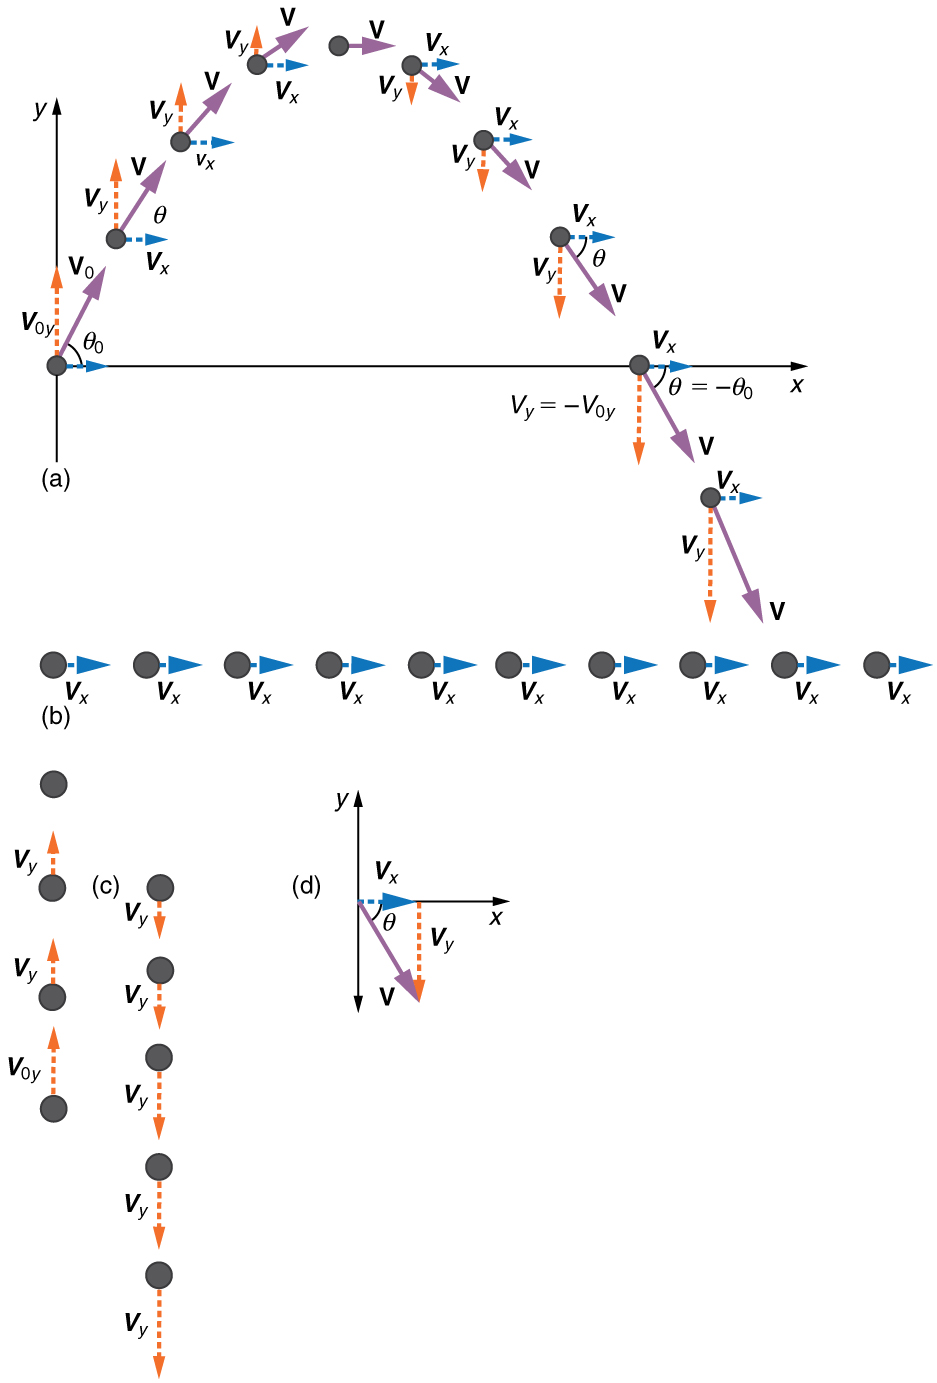
\includegraphics[width=0.45\textwidth,trim=0cm 15.5cm 3cm 0cm,clip=true]{figures/proj_motion.jpeg}
\caption{\label{fig:1} The velocity vector of a projectile in motion.}
\end{figure}

\end{document}